\documentclass{standalone}
\usepackage{tikz}
\usetikzlibrary{patterns, positioning}
\usepackage[sfdefault]{ClearSans} %% option 'sfdefault' activates Clear Sans as the default text font
\usepackage[T1]{fontenc}

\begin{document}
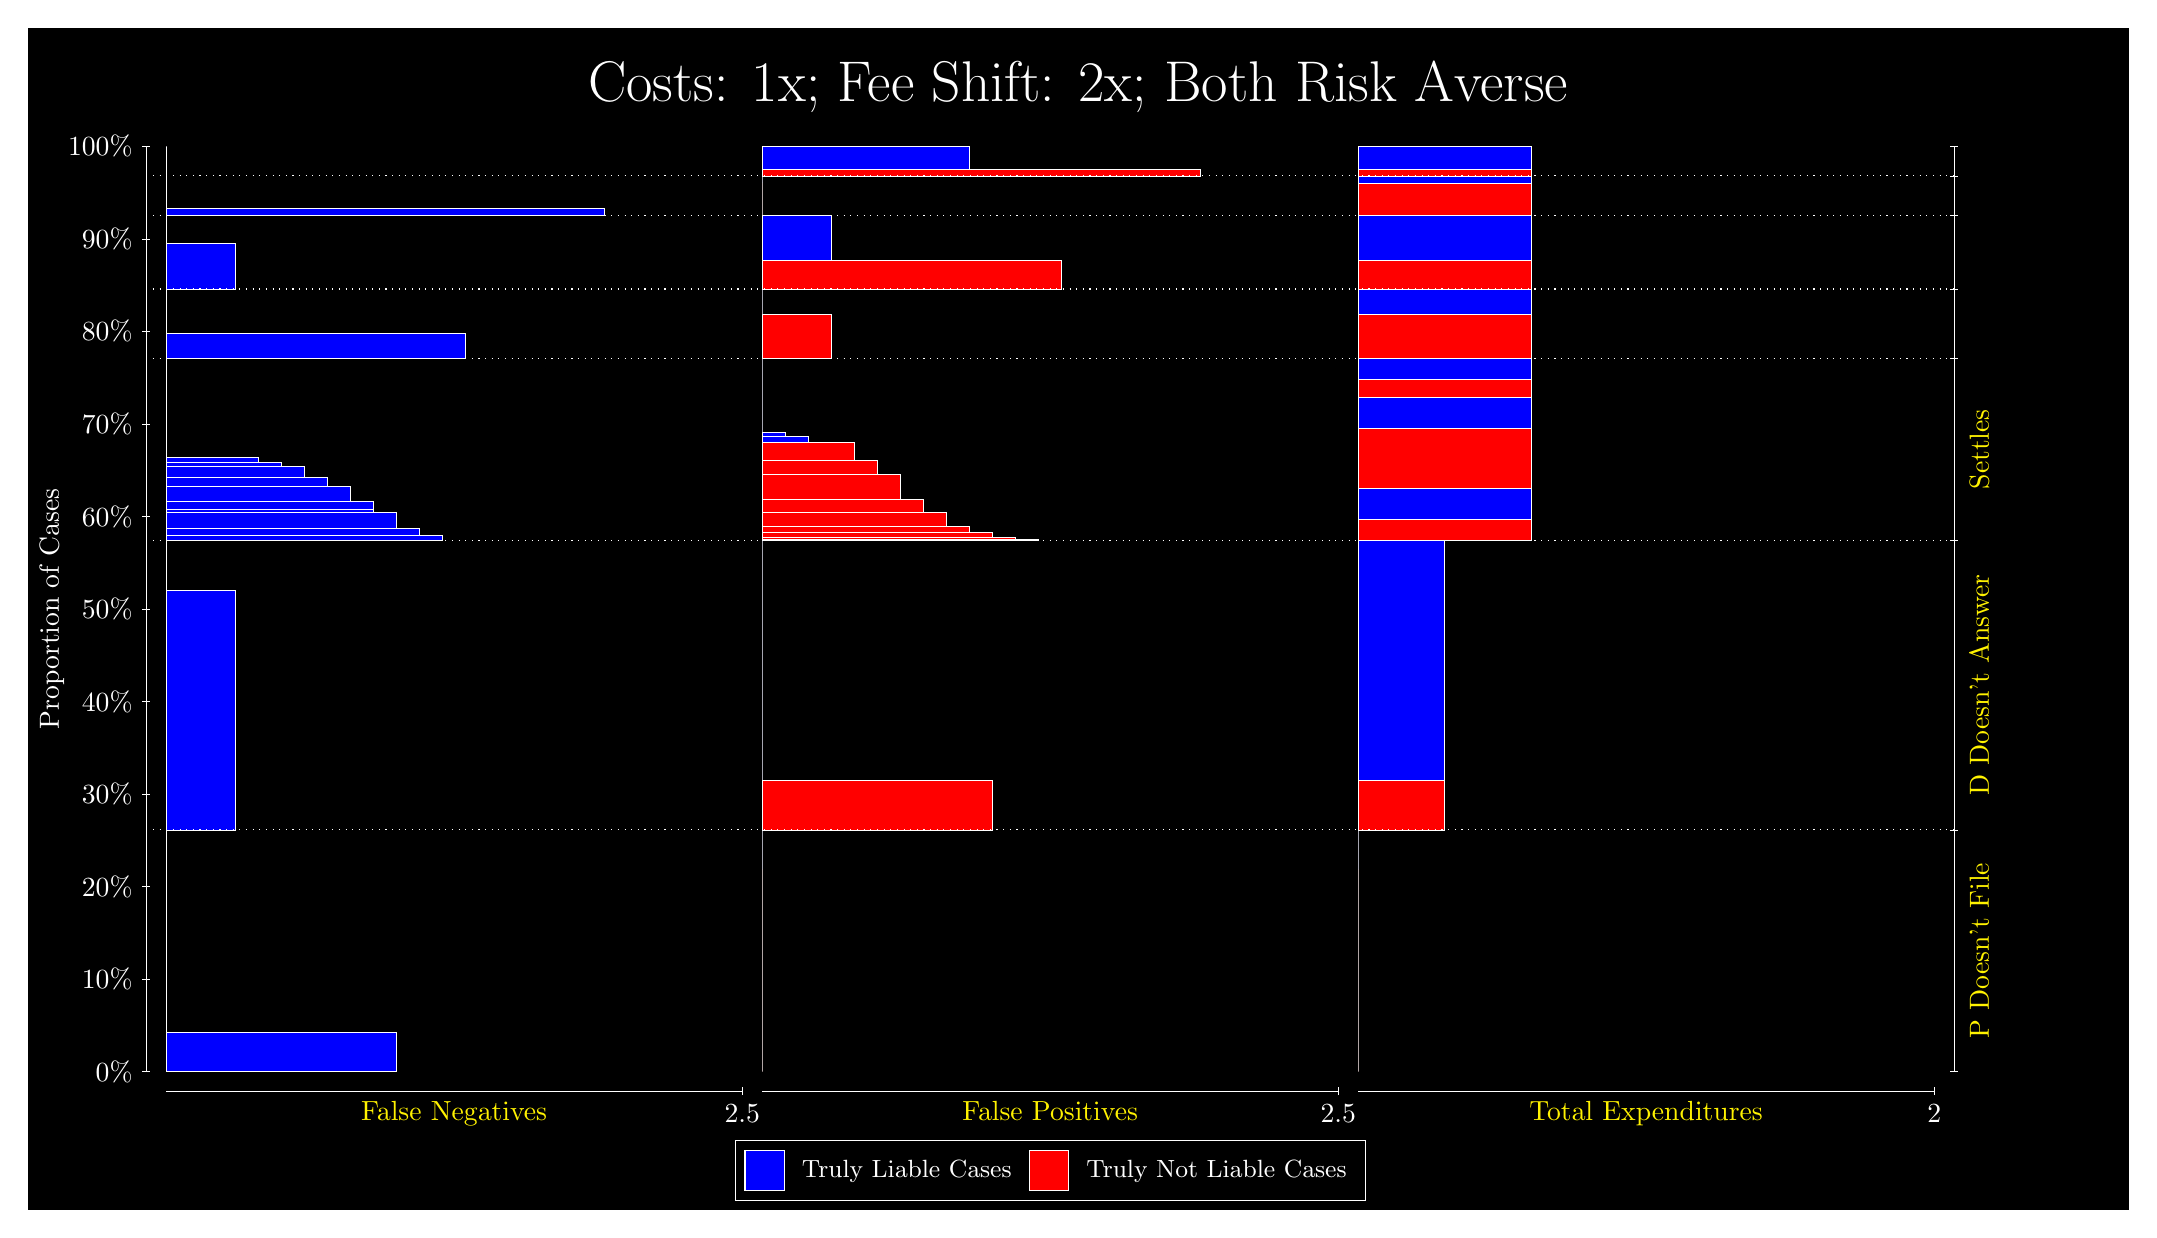
\begin{tikzpicture}
\draw[fill=black] (0,0) rectangle (26.667,15);
\draw[text=white] (0,13.5) rectangle (26.667,15) node[midway] {\huge Costs: 1x; Fee Shift: 2x; Both Risk Averse};
\draw[white, very thin] (1.5,1.75) -- (1.5,13.5);
\node[rotate=90, text=white, anchor=center] at (0.3, 7.625) {Proportion of Cases};
\draw[white, very thin] (1.45,1.75) -- (1.55,1.75);
\node[text=white, anchor=east] at (1.45, 1.75) {0\%};
\draw[white, very thin] (1.45,2.925) -- (1.55,2.925);
\node[text=white, anchor=east] at (1.45, 2.925) {10\%};
\draw[white, very thin] (1.45,4.1) -- (1.55,4.1);
\node[text=white, anchor=east] at (1.45, 4.1) {20\%};
\draw[white, very thin] (1.45,5.275) -- (1.55,5.275);
\node[text=white, anchor=east] at (1.45, 5.275) {30\%};
\draw[white, very thin] (1.45,6.45) -- (1.55,6.45);
\node[text=white, anchor=east] at (1.45, 6.45) {40\%};
\draw[white, very thin] (1.45,7.625) -- (1.55,7.625);
\node[text=white, anchor=east] at (1.45, 7.625) {50\%};
\draw[white, very thin] (1.45,8.8) -- (1.55,8.8);
\node[text=white, anchor=east] at (1.45, 8.8) {60\%};
\draw[white, very thin] (1.45,9.975) -- (1.55,9.975);
\node[text=white, anchor=east] at (1.45, 9.975) {70\%};
\draw[white, very thin] (1.45,11.15) -- (1.55,11.15);
\node[text=white, anchor=east] at (1.45, 11.15) {80\%};
\draw[white, very thin] (1.45,12.325) -- (1.55,12.325);
\node[text=white, anchor=east] at (1.45, 12.325) {90\%};
\draw[white, very thin] (1.45,13.5) -- (1.55,13.5);
\node[text=white, anchor=east] at (1.45, 13.5) {100\%};

\draw[white, very thin] (24.457,1.75) -- (24.457,13.5);
\draw[white, very thin] (24.407,1.75) -- (24.507,1.75);
\node[anchor=west] at (24.407, 1.75) {};
\draw[white, very thin] (24.407,4.8197) -- (24.507,4.8197);
\node[anchor=west] at (24.407, 4.8197) {};
\draw[white, very thin] (24.407,8.4956) -- (24.507,8.4956);
\node[anchor=west] at (24.407, 8.4956) {};
\draw[white, very thin] (24.407,10.809) -- (24.507,10.809);
\node[anchor=west] at (24.407, 10.809) {};
\draw[white, very thin] (24.407,11.688) -- (24.507,11.688);
\node[anchor=west] at (24.407, 11.688) {};
\draw[white, very thin] (24.407,12.627) -- (24.507,12.627);
\node[anchor=west] at (24.407, 12.627) {};
\draw[white, very thin] (24.407,13.124) -- (24.507,13.124);
\node[anchor=west] at (24.407, 13.124) {};
\draw[white, very thin] (24.407,13.5) -- (24.507,13.5);
\node[anchor=west] at (24.407, 13.5) {};

\draw[white, very thin, fill=blue] (1.75,1.75) rectangle (4.6775,2.2478);
\draw[white, very thin, fill=red] (1.75,2.2478) rectangle (1.75,4.8197);
\draw[white, very thin, fill=blue] (1.75,4.8197) rectangle (2.6283,7.8625);
\draw[white, very thin, fill=red] (1.75,7.8625) rectangle (1.75,8.4956);
\draw[white, very thin, fill=blue] (1.75,8.4956) rectangle (5.2631,8.5607);
\draw[white, very thin, fill=blue] (1.75,8.5607) rectangle (4.9703,8.6535);
\draw[white, very thin, fill=blue] (1.75,8.6535) rectangle (4.6775,8.8522);
\draw[white, very thin, fill=blue] (1.75,8.8522) rectangle (4.3848,8.89);
\draw[white, very thin, fill=blue] (1.75,8.89) rectangle (4.3848,8.9905);
\draw[white, very thin, fill=blue] (1.75,8.9905) rectangle (4.092,9.1866);
\draw[white, very thin, fill=blue] (1.75,9.1866) rectangle (3.7993,9.2909);
\draw[white, very thin, fill=blue] (1.75,9.2909) rectangle (3.5065,9.4313);
\draw[white, very thin, fill=blue] (1.75,9.4313) rectangle (3.2138,9.4891);
\draw[white, very thin, fill=blue] (1.75,9.4891) rectangle (2.921,9.5566);
\draw[white, very thin, fill=red] (1.75,9.5566) rectangle (1.75,10.809);
\draw[white, very thin, fill=blue] (1.75,10.809) rectangle (5.5558,11.129);
\draw[white, very thin, fill=red] (1.75,11.129) rectangle (1.75,11.688);
\draw[white, very thin, fill=blue] (1.75,11.688) rectangle (2.6283,12.264);
\draw[white, very thin, fill=red] (1.75,12.264) rectangle (1.75,12.627);
\draw[white, very thin, fill=blue] (1.75,12.627) rectangle (7.3123,12.716);
\draw[white, very thin, fill=red] (1.75,12.716) rectangle (1.75,13.124);
\draw[white, very thin, fill=red] (1.75,13.124) rectangle (1.75,13.213);
\draw[white, very thin, fill=blue] (1.75,13.213) rectangle (1.75,13.5);
\draw[white, very thin, fill=red] (9.3189,1.75) rectangle (9.3189,4.3219);
\draw[white, very thin, fill=blue] (9.3189,4.3219) rectangle (9.3189,4.8197);
\draw[white, very thin, fill=red] (9.3189,4.8197) rectangle (12.246,5.4528);
\draw[white, very thin, fill=blue] (9.3189,5.4528) rectangle (9.3189,8.4956);
\draw[white, very thin, fill=red] (9.3189,8.4956) rectangle (12.832,8.5156);
\draw[white, very thin, fill=red] (9.3189,8.5156) rectangle (12.539,8.5406);
\draw[white, very thin, fill=red] (9.3189,8.5406) rectangle (12.246,8.6034);
\draw[white, very thin, fill=red] (9.3189,8.6034) rectangle (11.954,8.6743);
\draw[white, very thin, fill=red] (9.3189,8.6743) rectangle (11.661,8.8529);
\draw[white, very thin, fill=red] (9.3189,8.8529) rectangle (11.368,9.0148);
\draw[white, very thin, fill=red] (9.3189,9.0148) rectangle (11.075,9.3313);
\draw[white, very thin, fill=red] (9.3189,9.3313) rectangle (10.783,9.5091);
\draw[white, very thin, fill=red] (9.3189,9.5091) rectangle (10.49,9.7477);
\draw[white, very thin, fill=blue] (9.3189,9.7477) rectangle (9.9044,9.8151);
\draw[white, very thin, fill=blue] (9.3189,9.8151) rectangle (9.6116,9.8729);
\draw[white, very thin, fill=blue] (9.3189,9.8729) rectangle (9.3189,10.809);
\draw[white, very thin, fill=red] (9.3189,10.809) rectangle (10.197,11.367);
\draw[white, very thin, fill=blue] (9.3189,11.367) rectangle (9.3189,11.688);
\draw[white, very thin, fill=red] (9.3189,11.688) rectangle (13.125,12.05);
\draw[white, very thin, fill=blue] (9.3189,12.05) rectangle (10.197,12.627);
\draw[white, very thin, fill=red] (9.3189,12.627) rectangle (9.3189,13.035);
\draw[white, very thin, fill=blue] (9.3189,13.035) rectangle (9.3189,13.124);
\draw[white, very thin, fill=red] (9.3189,13.124) rectangle (14.881,13.213);
\draw[white, very thin, fill=blue] (9.3189,13.213) rectangle (11.954,13.5);
\draw[white, very thin, fill=red] (16.888,1.75) rectangle (16.888,4.3219);
\draw[white, very thin, fill=blue] (16.888,4.3219) rectangle (16.888,4.8197);
\draw[white, very thin, fill=red] (16.888,4.8197) rectangle (17.986,5.4528);
\draw[white, very thin, fill=blue] (16.888,5.4528) rectangle (17.986,8.4956);
\draw[white, very thin, fill=red] (16.888,8.4956) rectangle (19.083,8.7621);
\draw[white, very thin, fill=blue] (16.888,8.7621) rectangle (19.083,9.1564);
\draw[white, very thin, fill=red] (16.888,9.1564) rectangle (19.083,9.9245);
\draw[white, very thin, fill=blue] (16.888,9.9245) rectangle (19.083,10.319);
\draw[white, very thin, fill=red] (16.888,10.319) rectangle (19.083,10.536);
\draw[white, very thin, fill=blue] (16.888,10.536) rectangle (19.083,10.809);
\draw[white, very thin, fill=red] (16.888,10.809) rectangle (19.083,11.367);
\draw[white, very thin, fill=blue] (16.888,11.367) rectangle (19.083,11.688);
\draw[white, very thin, fill=red] (16.888,11.688) rectangle (19.083,12.05);
\draw[white, very thin, fill=blue] (16.888,12.05) rectangle (19.083,12.627);
\draw[white, very thin, fill=red] (16.888,12.627) rectangle (19.083,13.035);
\draw[white, very thin, fill=blue] (16.888,13.035) rectangle (19.083,13.124);
\draw[white, very thin, fill=red] (16.888,13.124) rectangle (19.083,13.213);
\draw[white, very thin, fill=blue] (16.888,13.213) rectangle (19.083,13.5);
\draw[white, dotted] (1.5,4.8197) -- (24.457,4.8197);
\draw[white, dotted] (1.5,8.4956) -- (24.457,8.4956);
\draw[white, dotted] (1.5,10.809) -- (24.457,10.809);
\draw[white, dotted] (1.5,11.688) -- (24.457,11.688);
\draw[white, dotted] (1.5,12.627) -- (24.457,12.627);
\draw[white, dotted] (1.5,13.124) -- (24.457,13.124);
\draw[white, very thin] (1.75,1.5) -- (9.0689,1.5);
\node[text=yellow, anchor=north] at (5.4094, 1.5) {False Negatives};
\draw[white, very thin] (9.0689,1.45) -- (9.0689,1.55);
\node[text=white, anchor=north] at (9.0689, 1.45) {2.5};

\draw[white, very thin] (9.3189,1.5) -- (16.638,1.5);
\node[text=yellow, anchor=north] at (12.978, 1.5) {False Positives};
\draw[white, very thin] (16.638,1.45) -- (16.638,1.55);
\node[text=white, anchor=north] at (16.638, 1.45) {2.5};

\draw[white, very thin] (16.888,1.5) -- (24.207,1.5);
\node[text=yellow, anchor=north] at (20.547, 1.5) {Total Expenditures};
\draw[white, very thin] (24.207,1.45) -- (24.207,1.55);
\node[text=white, anchor=north] at (24.207, 1.45) {2};

\node[text=yellow, centered, rotate=90] at (24.777, 3.2849) {P Doesn't File};
\node[text=yellow, centered, rotate=90] at (24.777, 6.6576) {D Doesn't Answer};
\node[text=yellow, centered, rotate=90] at (24.777, 9.6521) {Settles};





\draw (12.978300999999998,1.5) node[draw=none] (baseCoordinate) {};
\begin{scope}[align=center]
        \matrix[scale=0.5, draw=white, below=0.5cm of baseCoordinate, nodes={draw}, column sep=0.1cm]{
            \node[rectangle, draw, minimum width=0.5cm, minimum height=0.5cm, fill=blue] {}; &
            \node[draw=none, font=\small, text=white] (B) {Truly Liable Cases}; &
            \node[rectangle, draw, minimum width=0.5cm, minimum height=0.5cm, fill=red] {}; &
            \node[draw=none, font=\small, text=white] (B) {Truly Not Liable Cases}; \\
            };
\end{scope}

\end{tikzpicture}
\end{document}